\chapter{Molten Salt Reactor Modeling}% \label{cha:msr_modeling}
%% lit review goes here
Much of our knowledge about \Gls{msr}s come from experiements on a test reactor
called the \Gls{msre} conducted at \Gls{ornl} in the 1960s, which demonstrated
the viability of the \Gls{msr} concept for use in civillian power programs
\cite{haubenreich_experience_1970} \cite{rosenthal_molten-salt_1970}.
%% Give brief description of the MSRE
%% cite a bunch of MSRE ORNL work.

The \Gls{msre} reactor to this day remains one of the few \Gls{msr}s to operate.
%% Maybe briefly mention other historical MSRs?

As of writing this thesis, there are no \Gls{msr}s currently in operation; we
must rely on computational and/or surrogate models to further study \Gls{msr}
physics. The \Gls{msre} is a popular choice for computational models due to the
availability of experimental data to compare results against. For example,
Roelofs et al used the system thermal hydraulics code SPECTRA to model steady
state parameters of the fuel-salt, \Gls{dnp} drift, and various fission product
behaviors in comparison with actual MSRE data \cite{roelofs_molten_2021}.
Podila et al performed a \Gls{cfd} simulation of the \Gls{msre} core to
investigate the ability of \Gls{cfd} to predict 3D effects in this kind of
reactor\cite{podila_cfd_2019}. 
%cite some MSRE studies
In addtion to the \Gls{msre}, the \Gls{msfr}\cite{merle-lucotte_launching_2011}
and \Gls{msbr}\cite{robertson_conceptual_1971} conceptual reactors are well
developed and are actively used in research. Park et al performed a whole core
analysis of the \Gls{msbr} using \MCNPSIX with additional depletion and
reprocessing using \CINDERNINETY and a custom Python script \cite{park_whole_2015}.
Aufiero et al extended \SerpentTWO with online fuel reprocessing capabilities to
study depletion in the \Gls{msfr} \cite{aufiero_extended_2013}.

These efforts illustrate that \Gls{msr} modeling encompasses a wide range of
physics domains.

\section{Modeling depletion in MSRs} Recall in Sections
\ref{sec:molten_salt_reactors} and \ref{sec:msr_codes} we introduced the
concepts of fuel depletion and removal and feed processes, and established the
importance of modeling fuel depletion to \Gls{msr} licensing. Depletion codes in
the past have shown good behavior when compared with depletion measurements from
commercial and research reactors; the \TRITON module in the \SCALE reactor physics
suite couples \SCALE's neutron transport solver (\Shift) and bateman equation
solver (\ORIGEN) to get accurate depletion for various reactor core geometries
\cite{dehart_reactor_2011}; The \SerpentTWO monte carlo particle transport code
also has fuel depletion capabilities \cite{leppanen_burnup_2009}. More recently,
OpenMC version 0.11 added support for fuel depletion and shows good agreement
with Serpent 2\cite{romano_depletion_2021}. 

Depletion simulations on \Gls{msr}s are difficult to verify through direct
measurement due to the lack of a physically operating reactor. Even so,
simulations will give us a good idea of what kinds of nuclides we can expect to
show up. Table \ref{tab:msr_depletion_tools} summarizes some currently available
software tools that can model depletion in \Gls{msr}s\footnote{additional works
like Aufiero et al \cite{aufiero_extended_2013}, while notable and relevant,
are bespoke modifications to currently existing software, and so cannot
truly be considered ``available'' until the modifications become part of the
software}.

\begin{table}[htpb] 
    \centering 
    \caption{Software tools that can model \Gls{msr} depletion with fuel reprocessing} 
    \label{tab:msr_depletion_tools}
    \begin{tabulary}{\linewidth}{|C|C|C|C|} 
        \hline
        Software tool & Description & Reprocessing scheme & Citation\\
        \hline 
        \ADDER & Interface code with internal depletion capabilities & Component-based continuous & \cite{nelson_molten_2021}\\
        \hline
        \SCALE & Suite code & Continuous & \cite{betzler_molten_2019}\\
        \hline 
        \SaltProc & Interface code & Component-based batch-wise & \cite{rykhlevskii_saltproc_2018}\\
        \hline 
    \end{tabulary}
\end{table}

\SaltProc has been used to perform lifetime depletion analysis on full-core models
of the \Gls{msbr}\cite{rykhlevskii_modeling_2019} and the Transatomic Power
MSR\cite{rykhlevskii_fuel_2020}. As seen in Figure \ref{fig:msbr_spectrum_comp},
the BOL and EOL neutron flux spectra for the MSBR results qualitatively matches those
reported Park et. al \cite{park_whole_2015}.\footnote{it shold be noted that Rykhlevskii
claims the results for the neuton flux spectra ``are in good agreement'' with those
reported by the original MSBR report \cite{robertson_conceptual_1971}, however the
neutron flux spectra reported in Robertson et al is unnormalized and tabulated, and
much the lower energy groups range}

\begin{figure}[htpb]
    \centering
    \subfloat[][]{
        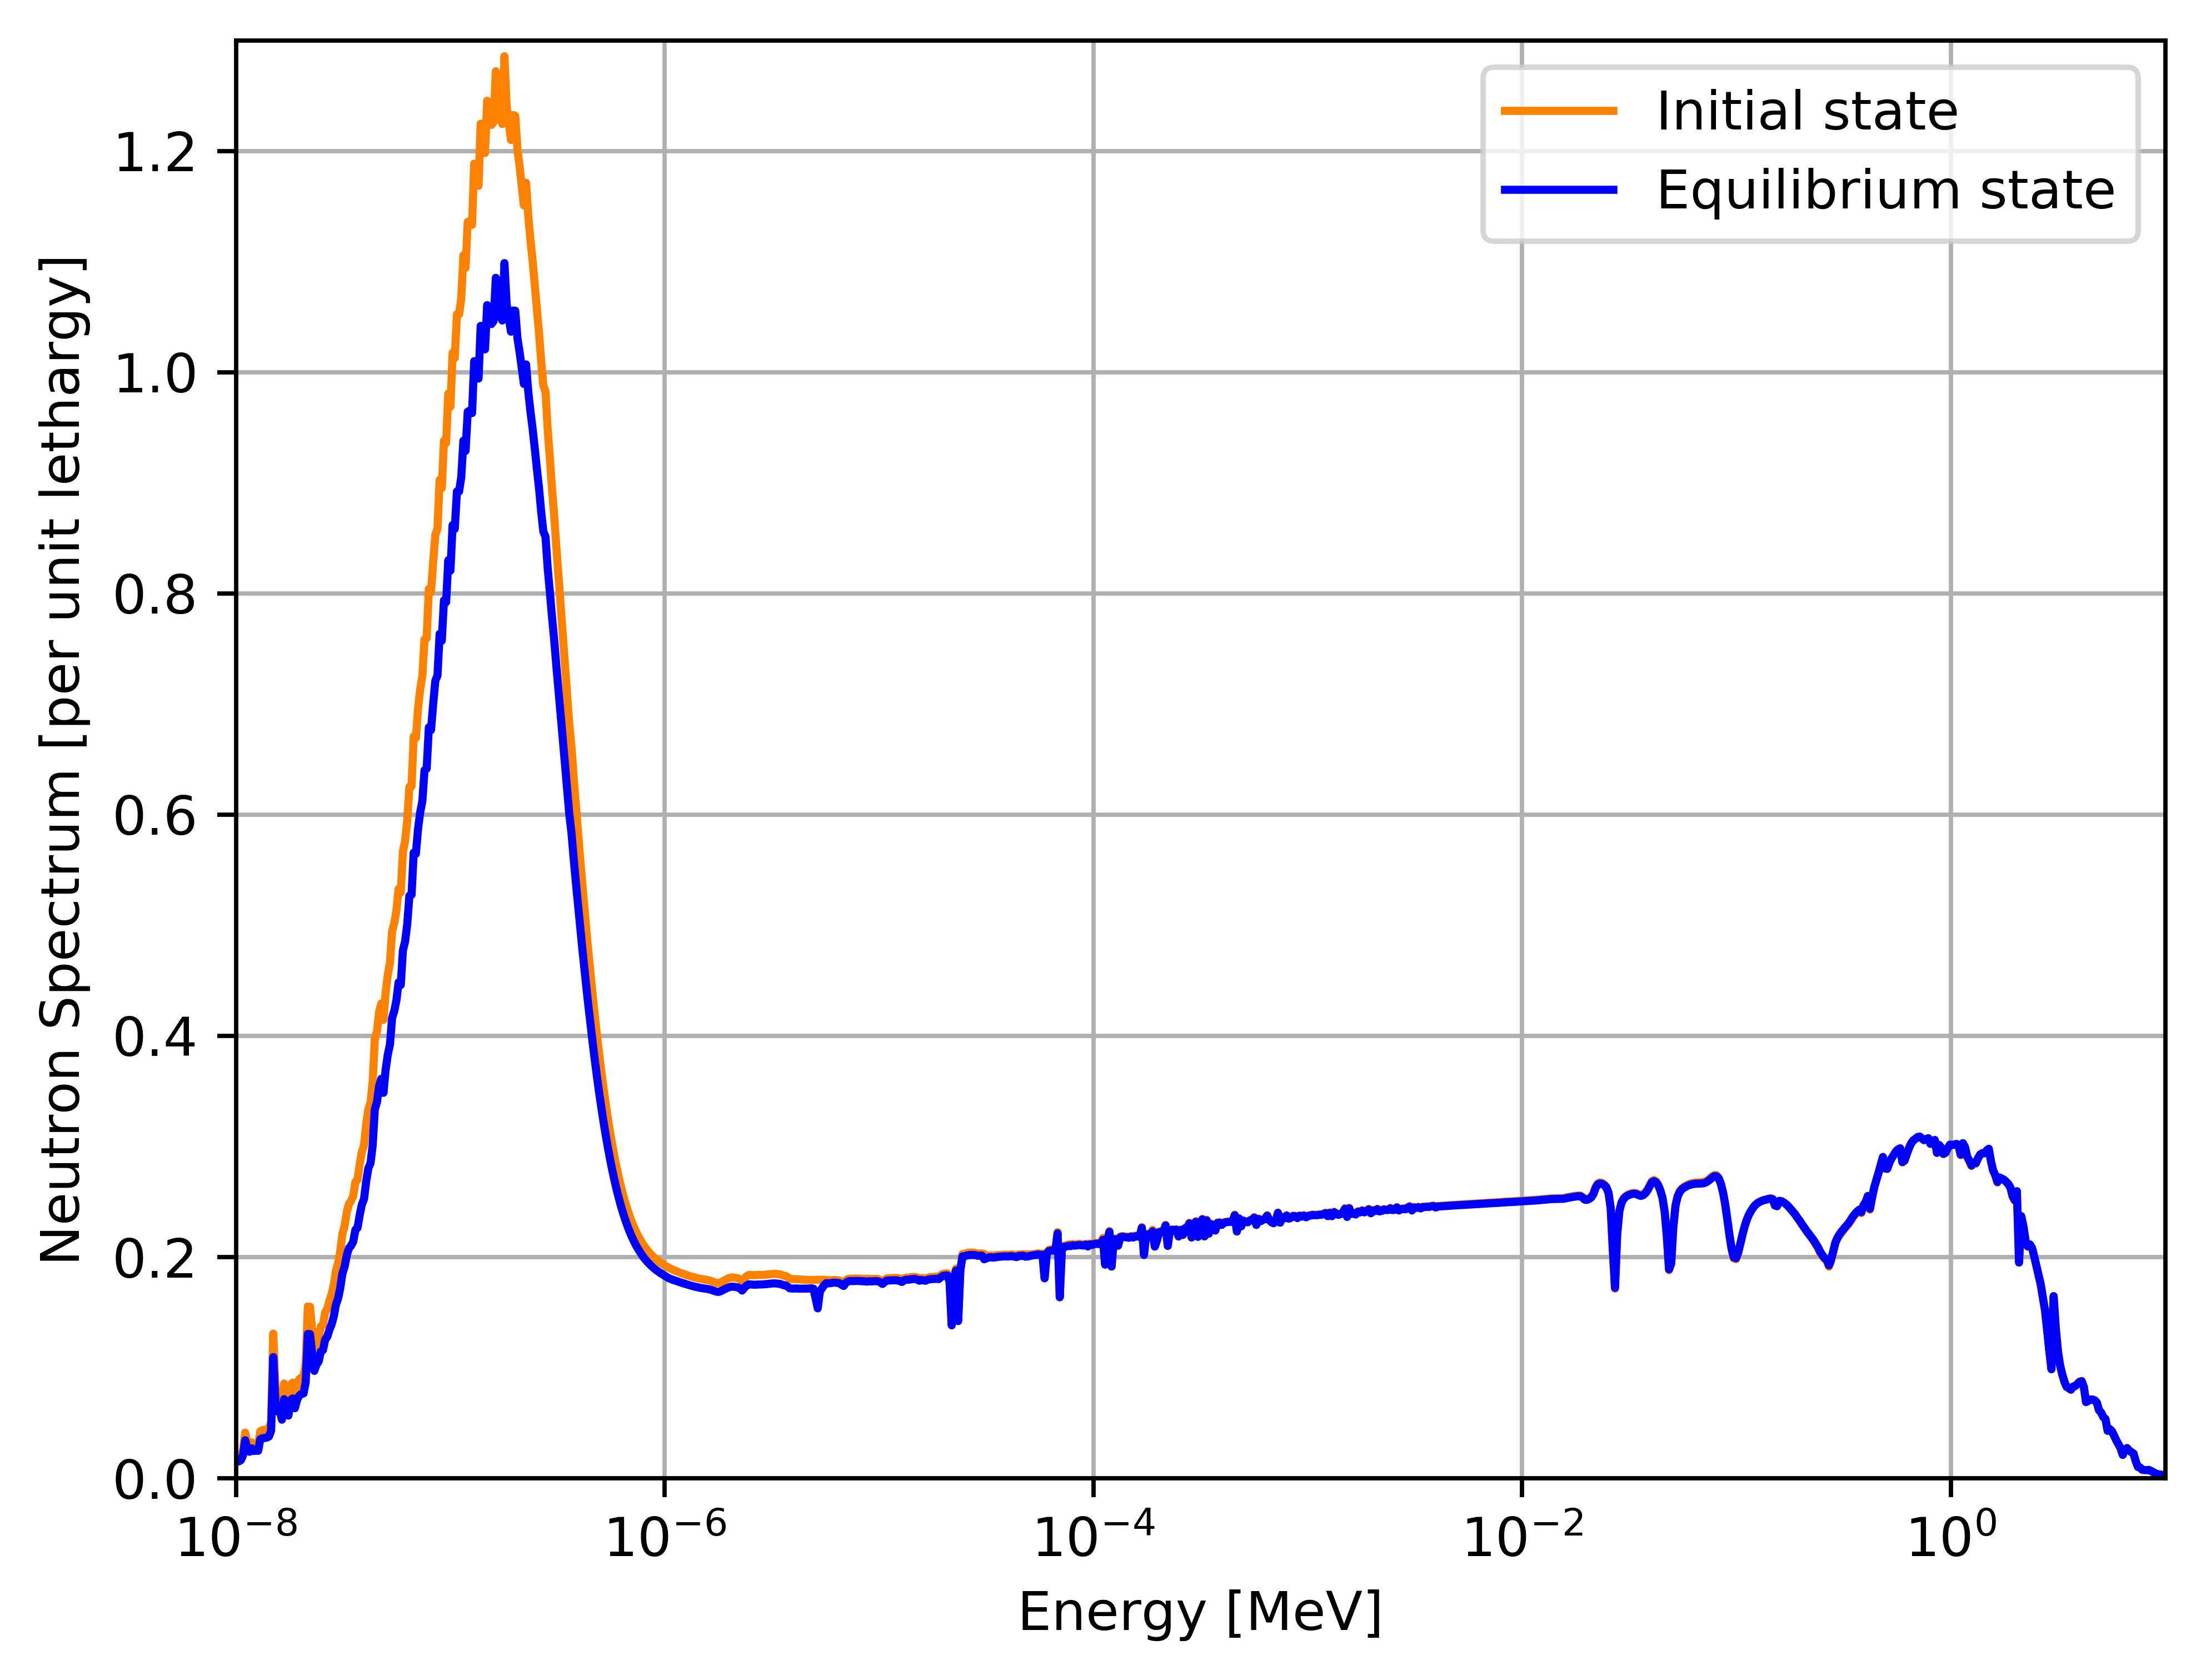
\includegraphics[width=0.5\linewidth]{figs/ch2/msbr_spectrum-rykhlevskii.png}
        \label{fig:msbr_spectrum_sub1}
                 }
    \subfloat[][]{
        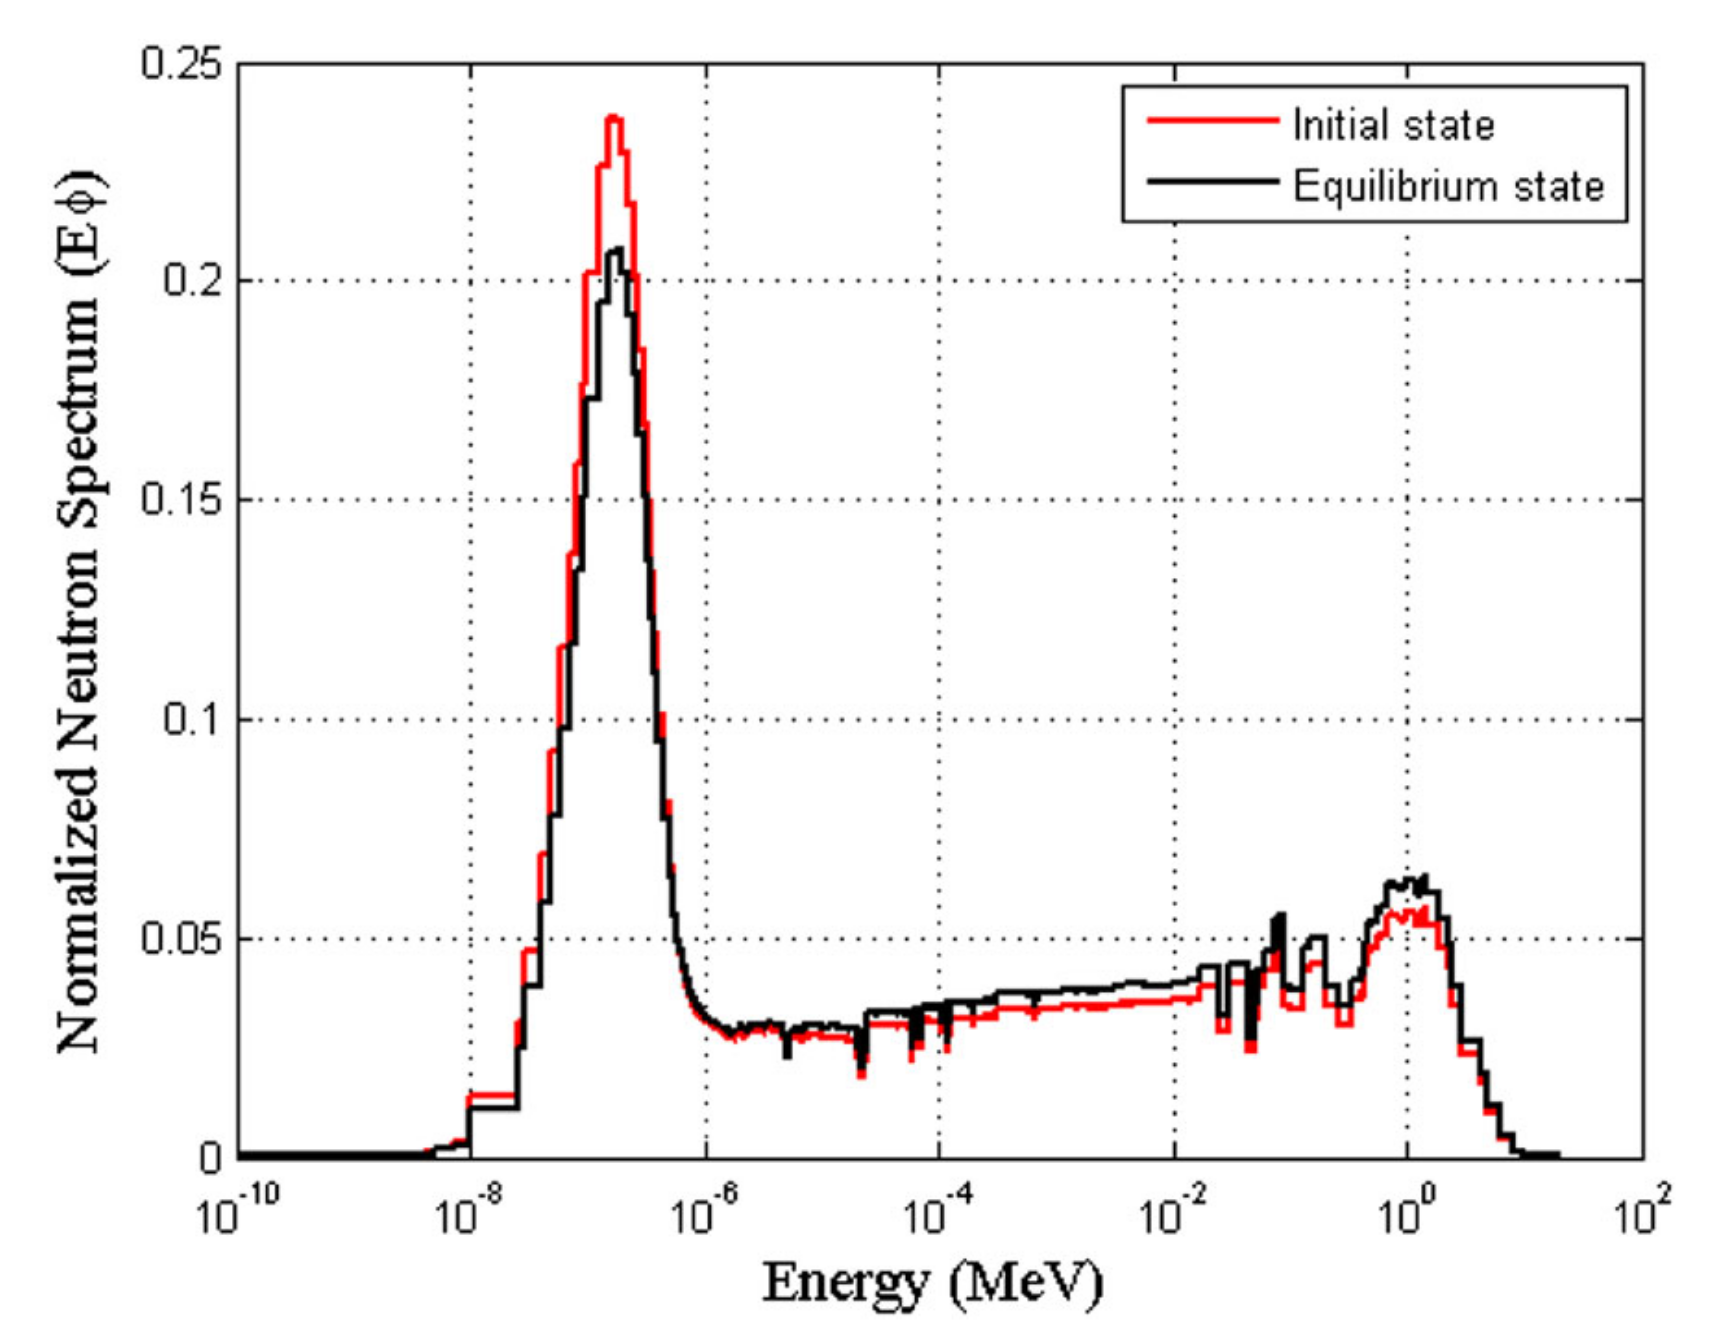
\includegraphics[width=0.5\linewidth]{figs/ch2/msbr_spectrum-park.png}
        \label{fig:msbr_spectrum_sub2}
                 }
    \caption[Side-by-side results of MSBR spectra between Ryhklevskii et al (2019) and Park et al (2015)]{
    \subref{fig:msbr_spectrum_sub1} Neutron flux energy spectrum at
    initial and equilibrium states normalized by unit lethargy. Reproduced
    from \cite{rykhlevskii_modeling_2019}; \subref{fig:msbr_spectrum_sub2}
    Neutron spectrum at initial and equilibirum states. Reproduced from
    \cite{park_whole_2015}}
    \label{fig:msbr_spectrum_comp}
\end{figure}
% in andrei's paper he makes several claims about good agreement with the MSBR results in the Robertson report, but I have been unable to find said results in that report

%TODO: Compare some of the reported numbers for flux magnitude against andrei's figures in his papers/thesis

Rykhlevskii compared the TAP MSR results against an \Gls{ornl} technical report
on neutronic performance of the same reactor\cite{betzler_assessment_2017} using
identical cross section libraries and model parameters wherever possible.
Betzler et. al. used the ChemTriton\cite{betzler_molten_2017} interface code
that perfoms batch-wise reprocessing using the \SCALE suite for coupled
transport-depletion. ChemTriton was extended to use the
Shift\cite{davidson_nuclide_2018} monte carlo particle transport tool for 3D
neutron transport and depletion \footnote{at the time of publication, Shift had
not yet been incorporated into SCALE}. As seen in Figure \ref{fig:tap_spectra}, neutron flux
spectra results between the SaltProc and ChemTriton simulations showed decent
agreement.

\begin{figure}[htpb]
    \centering
    \subfloat[][]{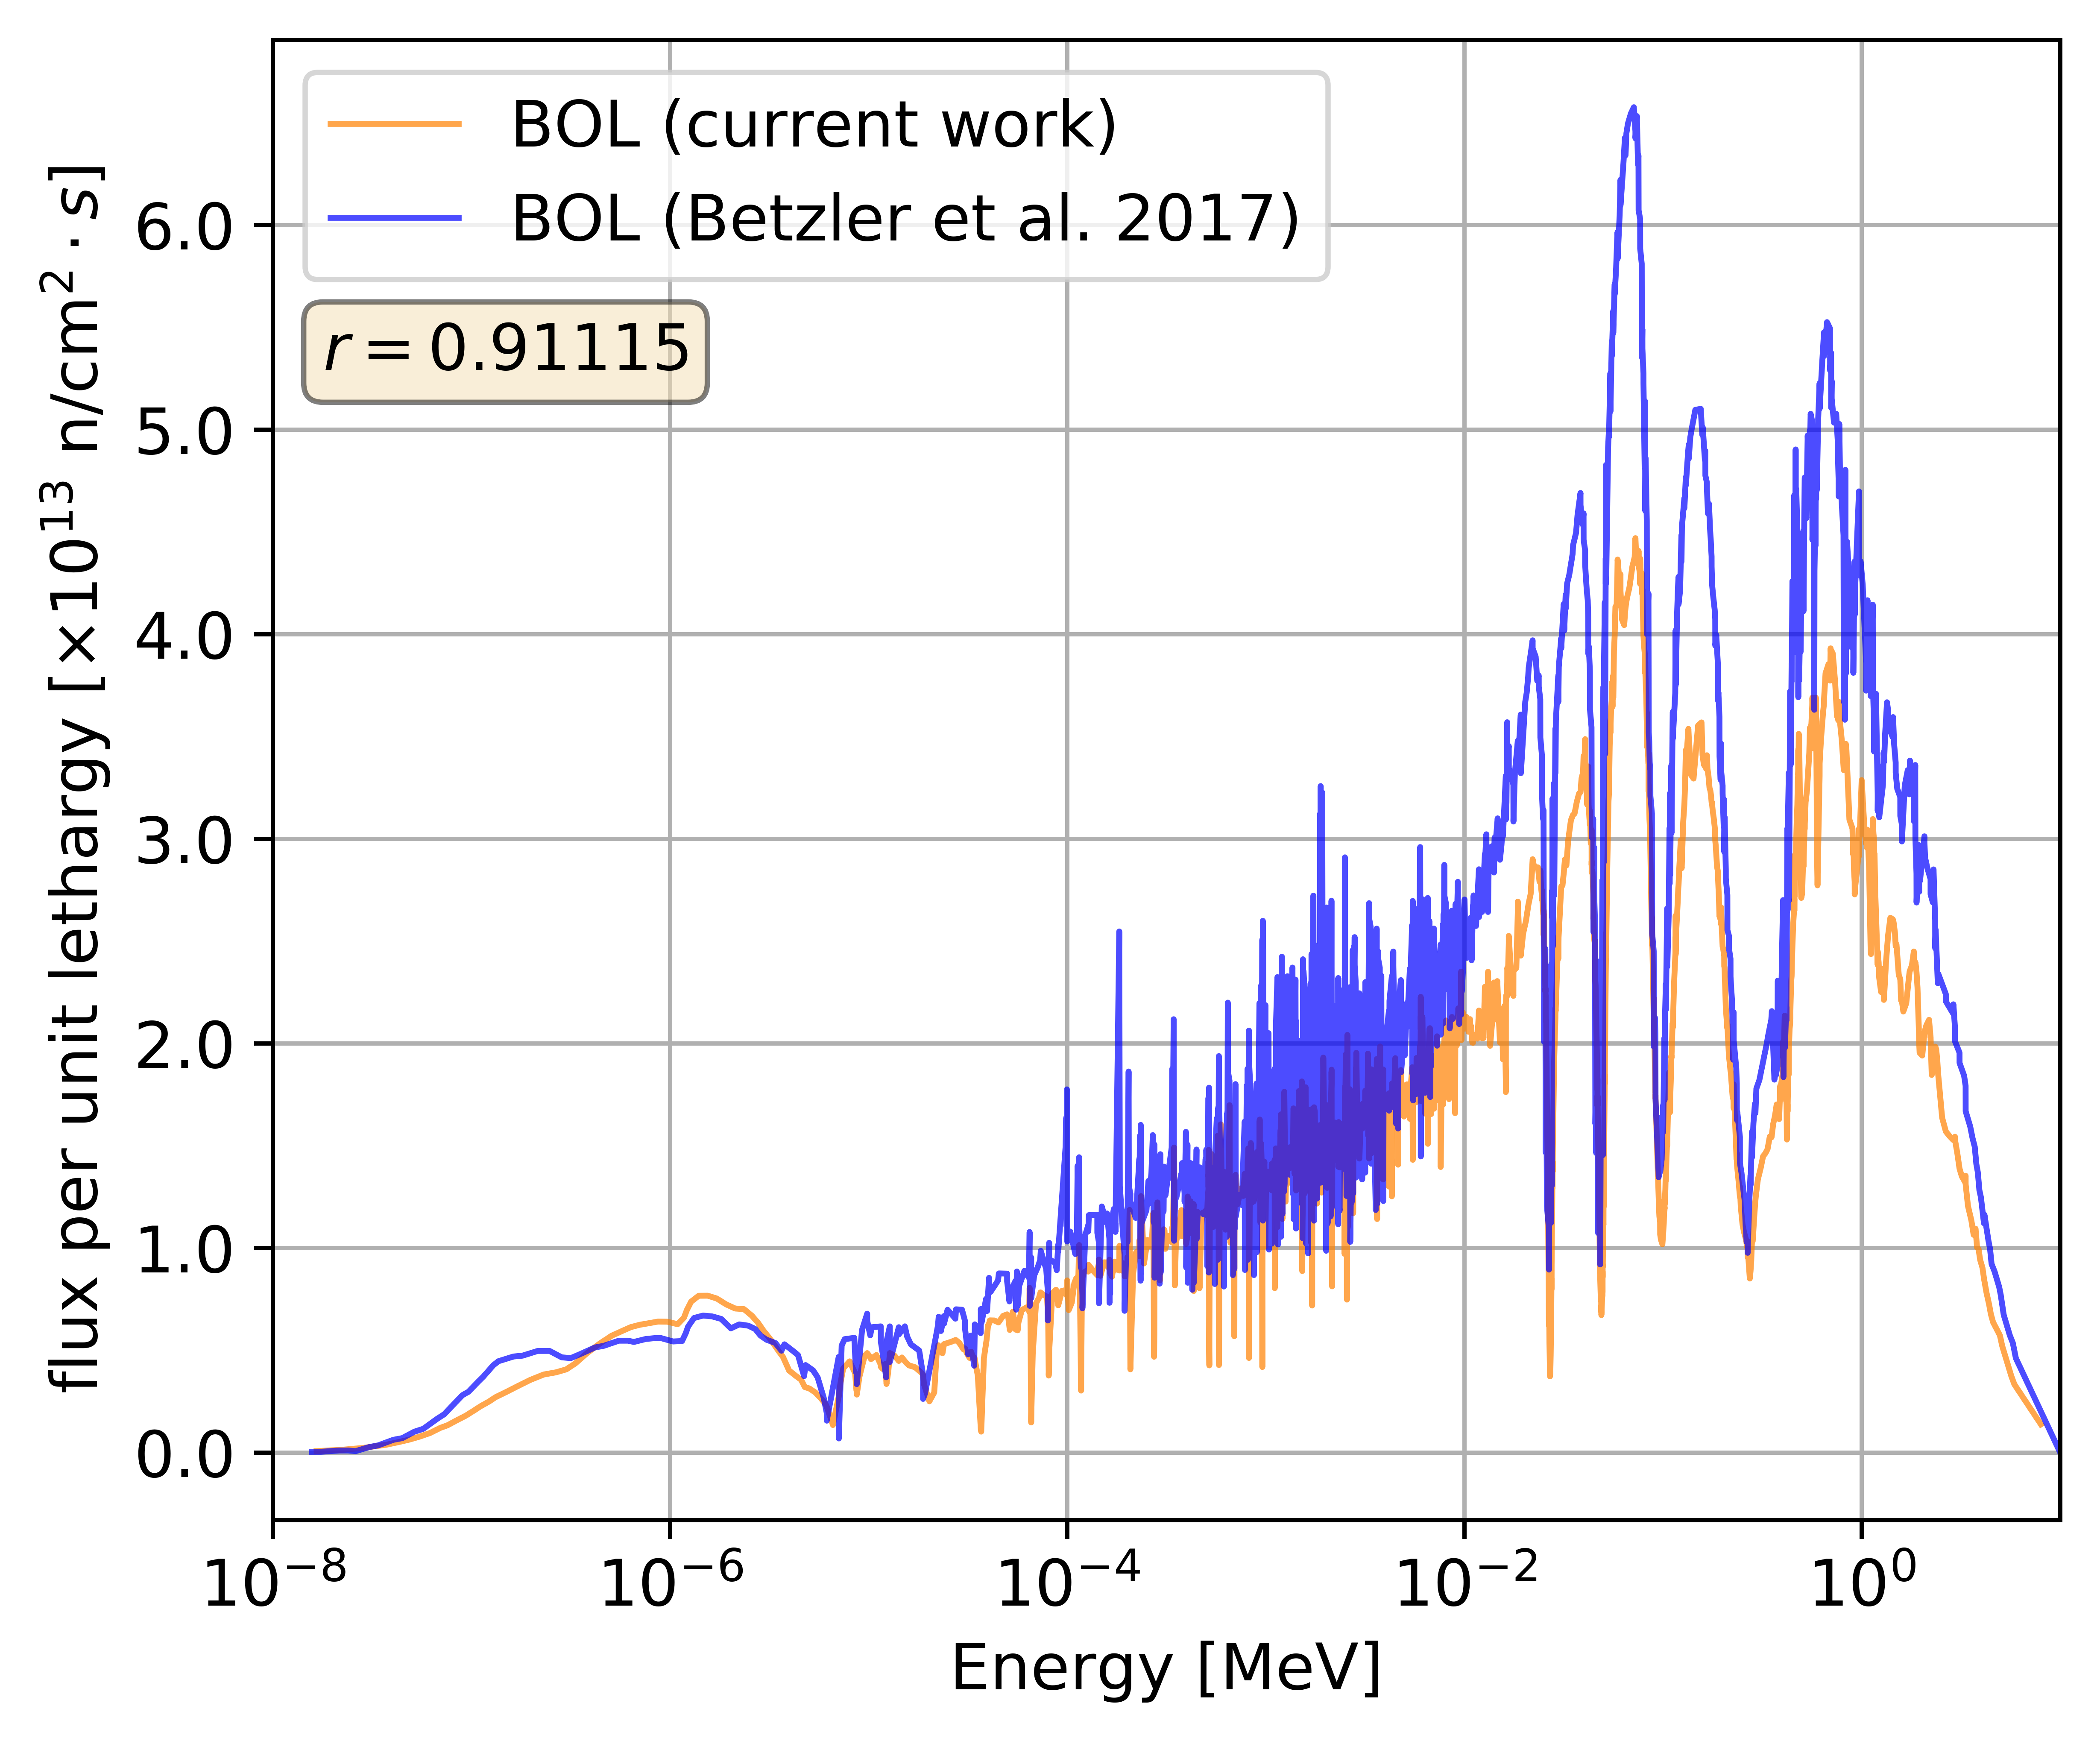
\includegraphics[width=0.5\linewidth]{figs/ch2/ben_spec_bol.png}
    \label{fig:tap_spectrum_bol}}
    \subfloat[][]{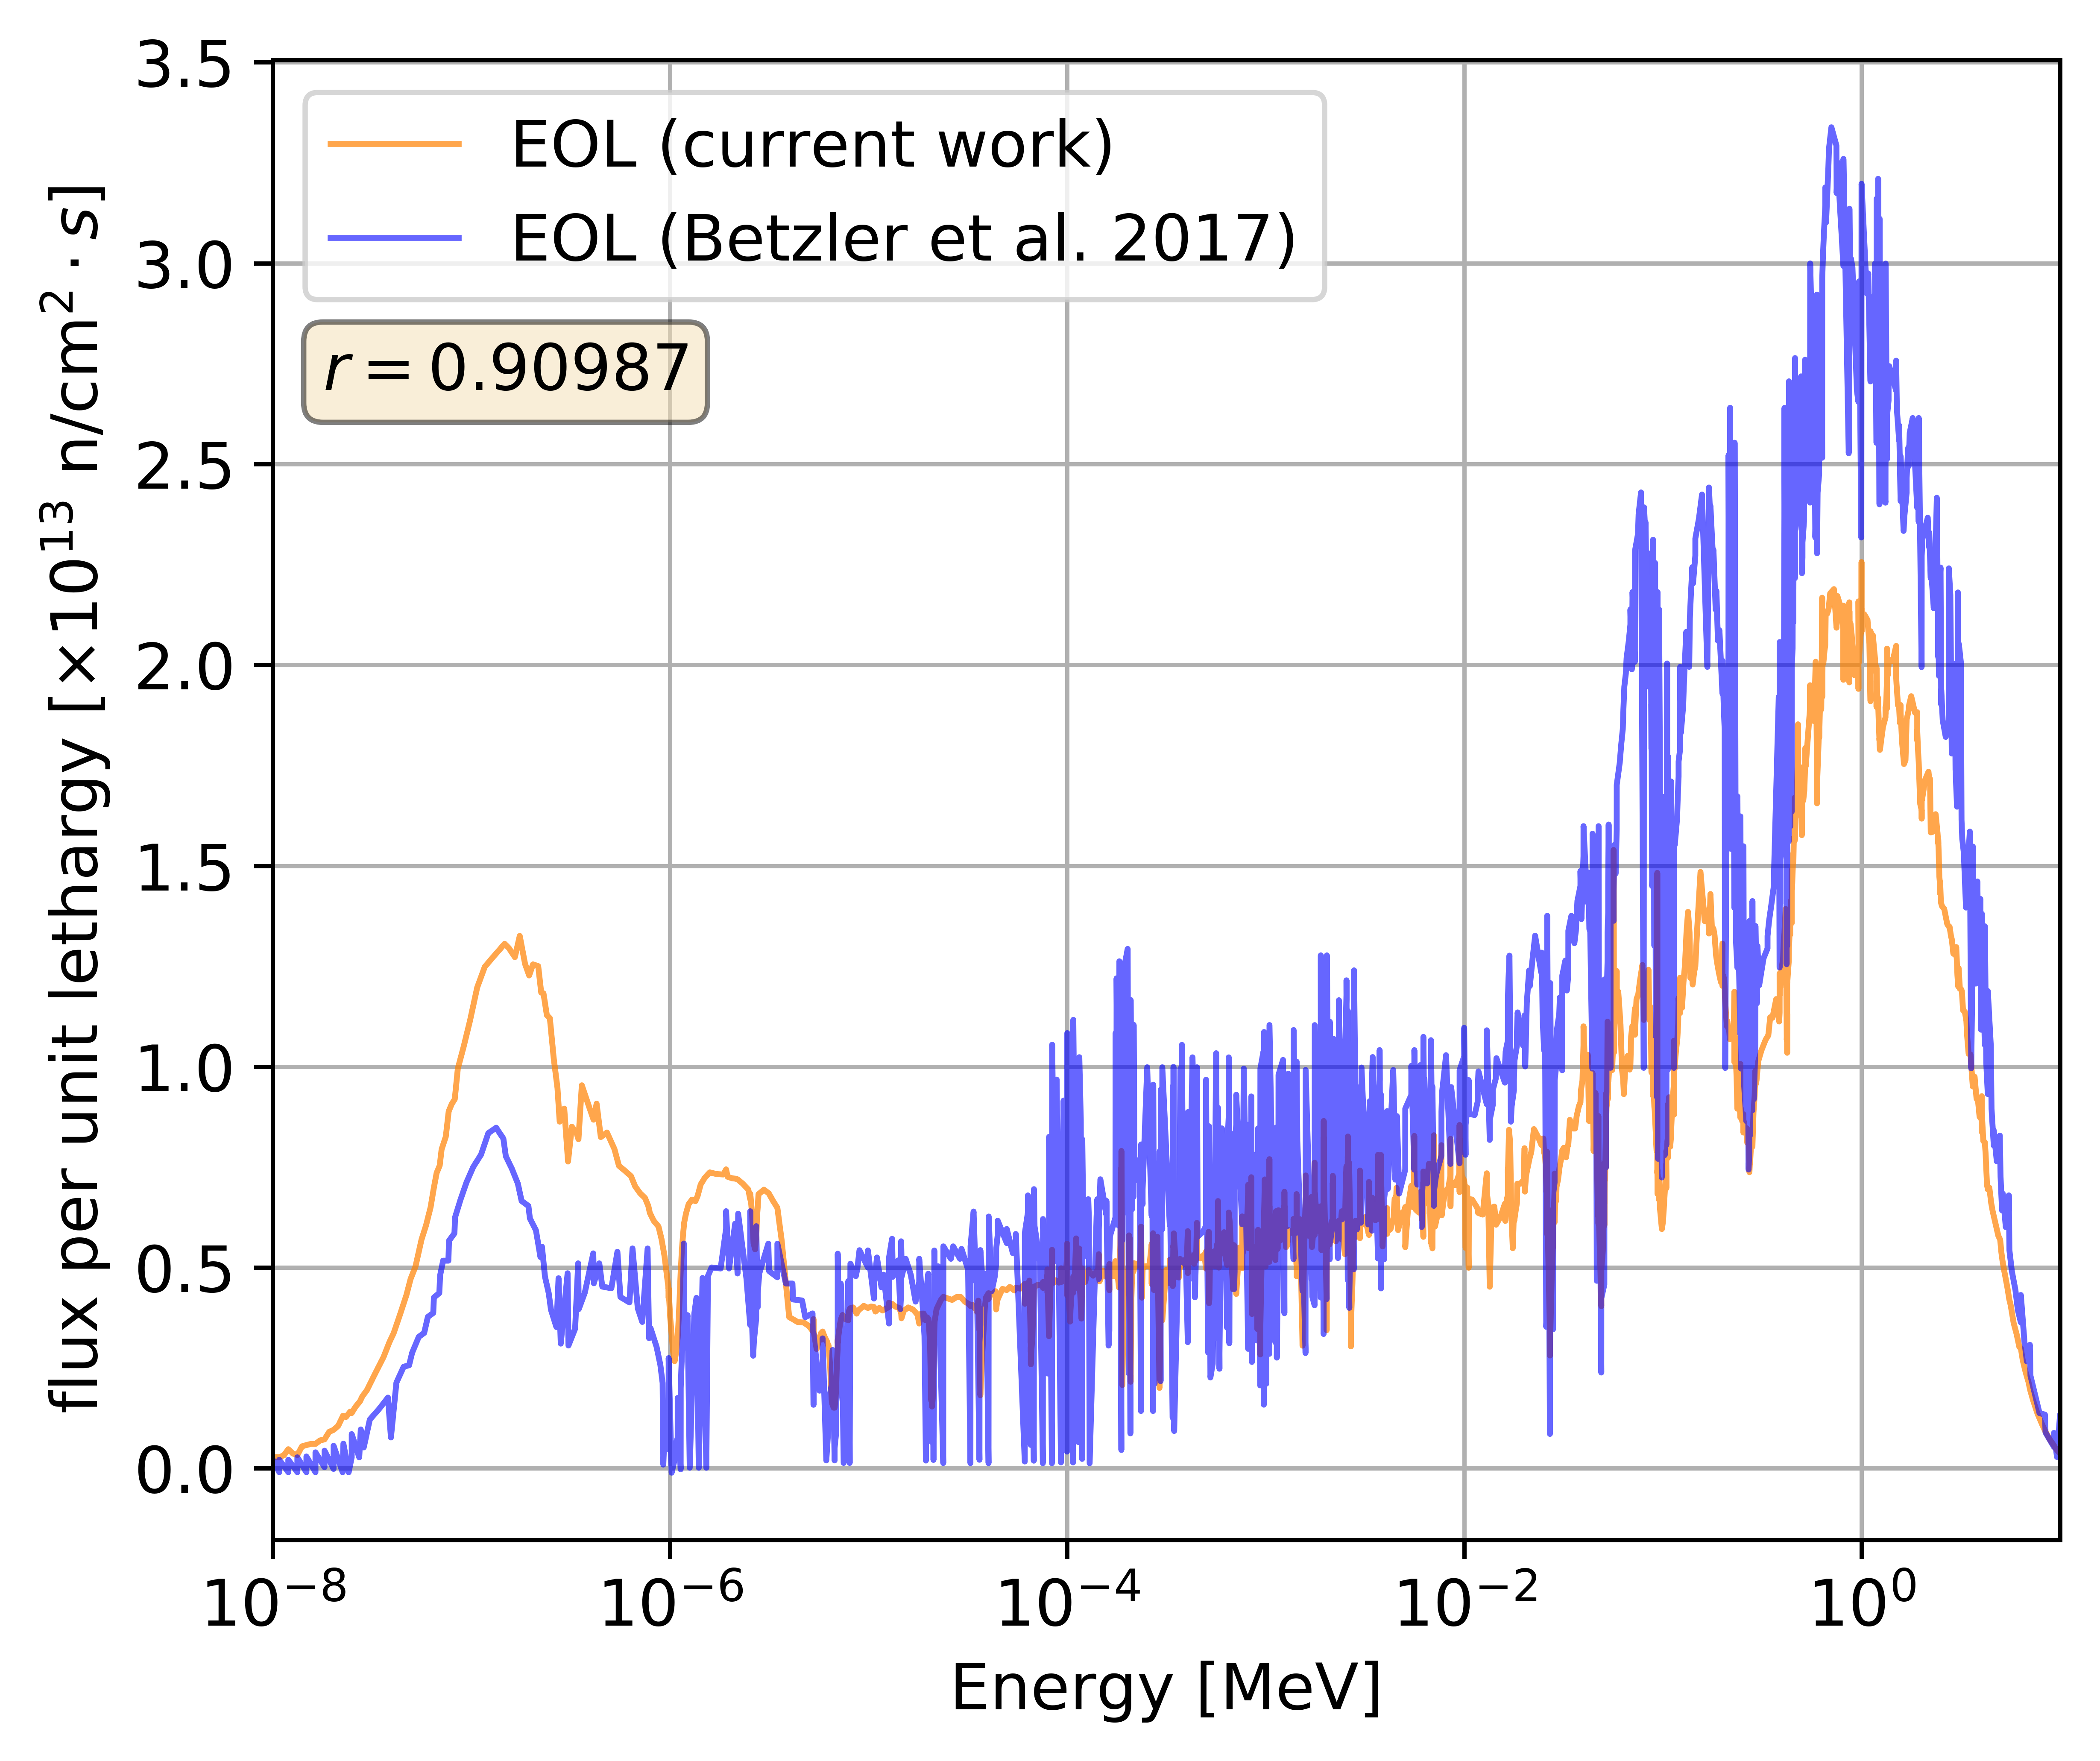
\includegraphics[width=0.5\linewidth]{figs/ch2/ben_spec_eol.png}
    \label{fig:tap_spectrum_eol}}
    \caption[Comparative results of TAP MSR flux spectra at BOL and EOL]{
        Comparative results of TAP MSR flux spectra at BOL and EOL:
        \ref{fig:tap_spectrum_bol} BOL;
        \ref{fig:tap_spectrum_eol} EOL;
        Both figures reproduced from \cite{rykhlevskii_fuel_2020}
    }
    \label{fig:tap_spectra}
\end{figure}


\subsection{Practical differences in continuous and batch-wise reprocessing}
We defined continuous and batch-wise reprocessing and discussed their
theoretical differences in in Section \ref{sec:msr_codes}. There are also some
practical implications on problem setup and results between these two methods.
Betzler, et. al. (2019) \cite{betzler_molten_2019} perfomed a code-to-code
comparsion between new functionality added to the \ORIGEN and \SCALE/\TRITON codes
for simulating depletion in \Gls{msr}s with continuous reprocessing, and the
older \ChemTriton(cite) interface code that perfoms batch-wise reprocessing using
the \SCALE suite for coupled transport-depletion. They found that the two
reprocessing schemes generally produced similar results with the following
caveats:
\begin{enumerate}
    \item $k_{\infty}$ for batch-wise reprocessing trends slightly lower than  continuous reprocessing. The authors claim this is due to \ChemTriton's {\it middlestep depletion method}. 
    \item The batch-wise method generally results in higher concentrations of nuclides. Notably, nuclides with short half lives, like \ce{^{135}Xe}, trends significantly higher in batch-wise reprocessing.
\end{enumerate}


\section{Differences between Serpent and OpenMC}
As mentioned in Section \ref{sec:objectives}, a major objective of this thesis
is to implement support for \OpenMC's \verb.deplete. module. In this context,
I would like to discuss some of the differences between \OpenMC and \SerpentTWO.
The most in-depth discission of these differences that I have found are in
\cite{romano_depletion_2021}. I have tabulated the differences discussed in that
paper below.
\begin{table}[htpb] 
    \centering 
    \caption{Differences between OpenMC and Serpent} 
    \label{tab:mc_code_diffs}
    \begin{tabulary}{\linewidth}{|C|C|C|} 
        \hline
        Metric & OpenMC & Serpent \\ 
        \hline 
        Access & Open source, hosted on GitHub & Export controlled, code distributed by RSICC (USA), OECD/NEA\\
        \hline
        User interface & Python API & Manual writing of geometry, material, and settings files\\
        \hline 
        Handling of cross sections in between library temperatures & interpolation between neighboring temperatures & target motion-sampling \cite{viitanen_explicit_2012}\\
        \hline 
        Matrix exponential solver & IPF CRAM-48 & PDF CRAM-14 \\
        \hline
        Cross section file formate & HDF5 & ACE \\
        \hline
        S$(\alpha, \beta)$ representation & continuous & tabulated \\
        \hline
    \end{tabulary}
\end{table}
As mentioned earlier, Romano found good agreement between OpenMC depletion results and Serpent depletion results, but notes that one must take careful consideration of the data and internal settings to get good results between codes. Of note are the default energy release per fission of \ce{^{235}U} used for power normalization and capture branching ratios. We follow Romano's methodology to ensure data consitency in our comparative study.
%% talk about saltproc in it's current state, the gaps that exist
%% lead into discussion about why it's important to add openmc 
%% capabilities to SaltProc. Also mention the differnces in 
%% Serpent2 and OpenMC cross section handling and how this
%% adds capability to the SaltProc tool
